\documentclass[11pt,a4paper]{beamer}
\usepackage[latin1]{inputenc}
\usepackage[dutch]{babel}

\usepackage[absolute,overlay]{textpos}
\setlength{\TPHorizModule}{1mm}
\setlength{\TPVertModule}{1mm}

\author{Zeus WPI}

% Voor- en achtergrondkleurtjes
\definecolor{gray}{RGB}{56,56,56}
\setbeamercolor{background canvas}{bg=gray}
\setbeamercolor{normal text}{fg=white}
\setbeamercolor{block title}{fg=white}
% Verwijder navigatieknopjes
\beamertemplatenavigationsymbolsempty

% Randjes voor fbox's rond de afbeeldingen
\setlength{\fboxsep}{0pt}
\setlength{\fboxrule}{1pt}


\begin{document}

% Eerste slide met logo
\begin{frame}
  \includegraphics[width=\textwidth]{zeus_logo.pdf}\\[5mm]

  \hfill --- by Elo \&\& Noctua

\end{frame}
% Wat we doen
\begin{frame}
  \begin{textblock}{20}(10,25)
    {\Huge Activiteiten}
  \end{textblock}

  \pause
  \begin{textblock}{20}(50,45)
    \visible<2->{\Huge Projecten}
  \end{textblock}

  \pause
  \begin{textblock}{20}(90,65)
    \visible<3->{\Huge Sfeer}
  \end{textblock}

\end{frame}


% Activiteiten
\begin{frame}
  \begin{center}
    {\Huge Activiteiten}
  \end{center}

\end{frame}
%LAN
\begin{frame} 

  \begin{textblock}{60}(10,15)
    {\huge LAN Party}
  \end{textblock}

  \begin{textblock}{20}(22,40)
    \visible{\fbox{\includegraphics[width=235pt]{activiteit_lan.jpg}}}
  \end{textblock}

\end{frame}

%linux install
\begin{frame}

  \begin{textblock}{60}(10,15)
    {\huge Linux install party}
  \end{textblock}

  \begin{textblock}{20}(30,23)
    \visible{\includegraphics[width=200pt]{tux.png}}
  \end{textblock}
\end{frame}

%lessen
\begin{frame}

  \begin{textblock}{60}(10,15)
    {\huge Lessen}
  \end{textblock}

  \begin{textblock}{20}(30,30)
    \visible{\fbox{\includegraphics[width=180pt]{activiteit_latex.jpg}}}
  \end{textblock}
\end{frame}


% Projecten
\begin{frame}
  \begin{center}
    {\Huge Projecten}
  \end{center}
\end{frame}

\begin{frame}

  \begin{textblock}{60}(10,15)
    {\huge Hydra}
  \end{textblock}

  \begin{textblock}{20}(40,15)
    \visible{\fbox{\includegraphics[width=160pt]{project_hydra.png}}}
  \end{textblock}
\end{frame}

\begin{frame}

  \begin{textblock}{60}(10,15)
    {\huge Gandalf}
  \end{textblock}

  \begin{textblock}{20}(15,30)
    \visible{\fbox{\includegraphics[width=270pt]{project_gandalf.png}}}
  \end{textblock}
\end{frame}

\begin{frame}
  \begin{textblock}{60}(10,15)
    {\huge 12u loop}
  \end{textblock}
  \begin{textblock}{20}(25,30)
    \visible{\fbox{\includegraphics[width=230pt]{project_12ul.jpg}}}
  \end{textblock}
\end{frame}

\begin{frame}
  \begin{textblock}{60}(10,15)
    {\huge Slotmachien}
  \end{textblock}
  \begin{textblock}{20}(25,30)
    \visible{\fbox{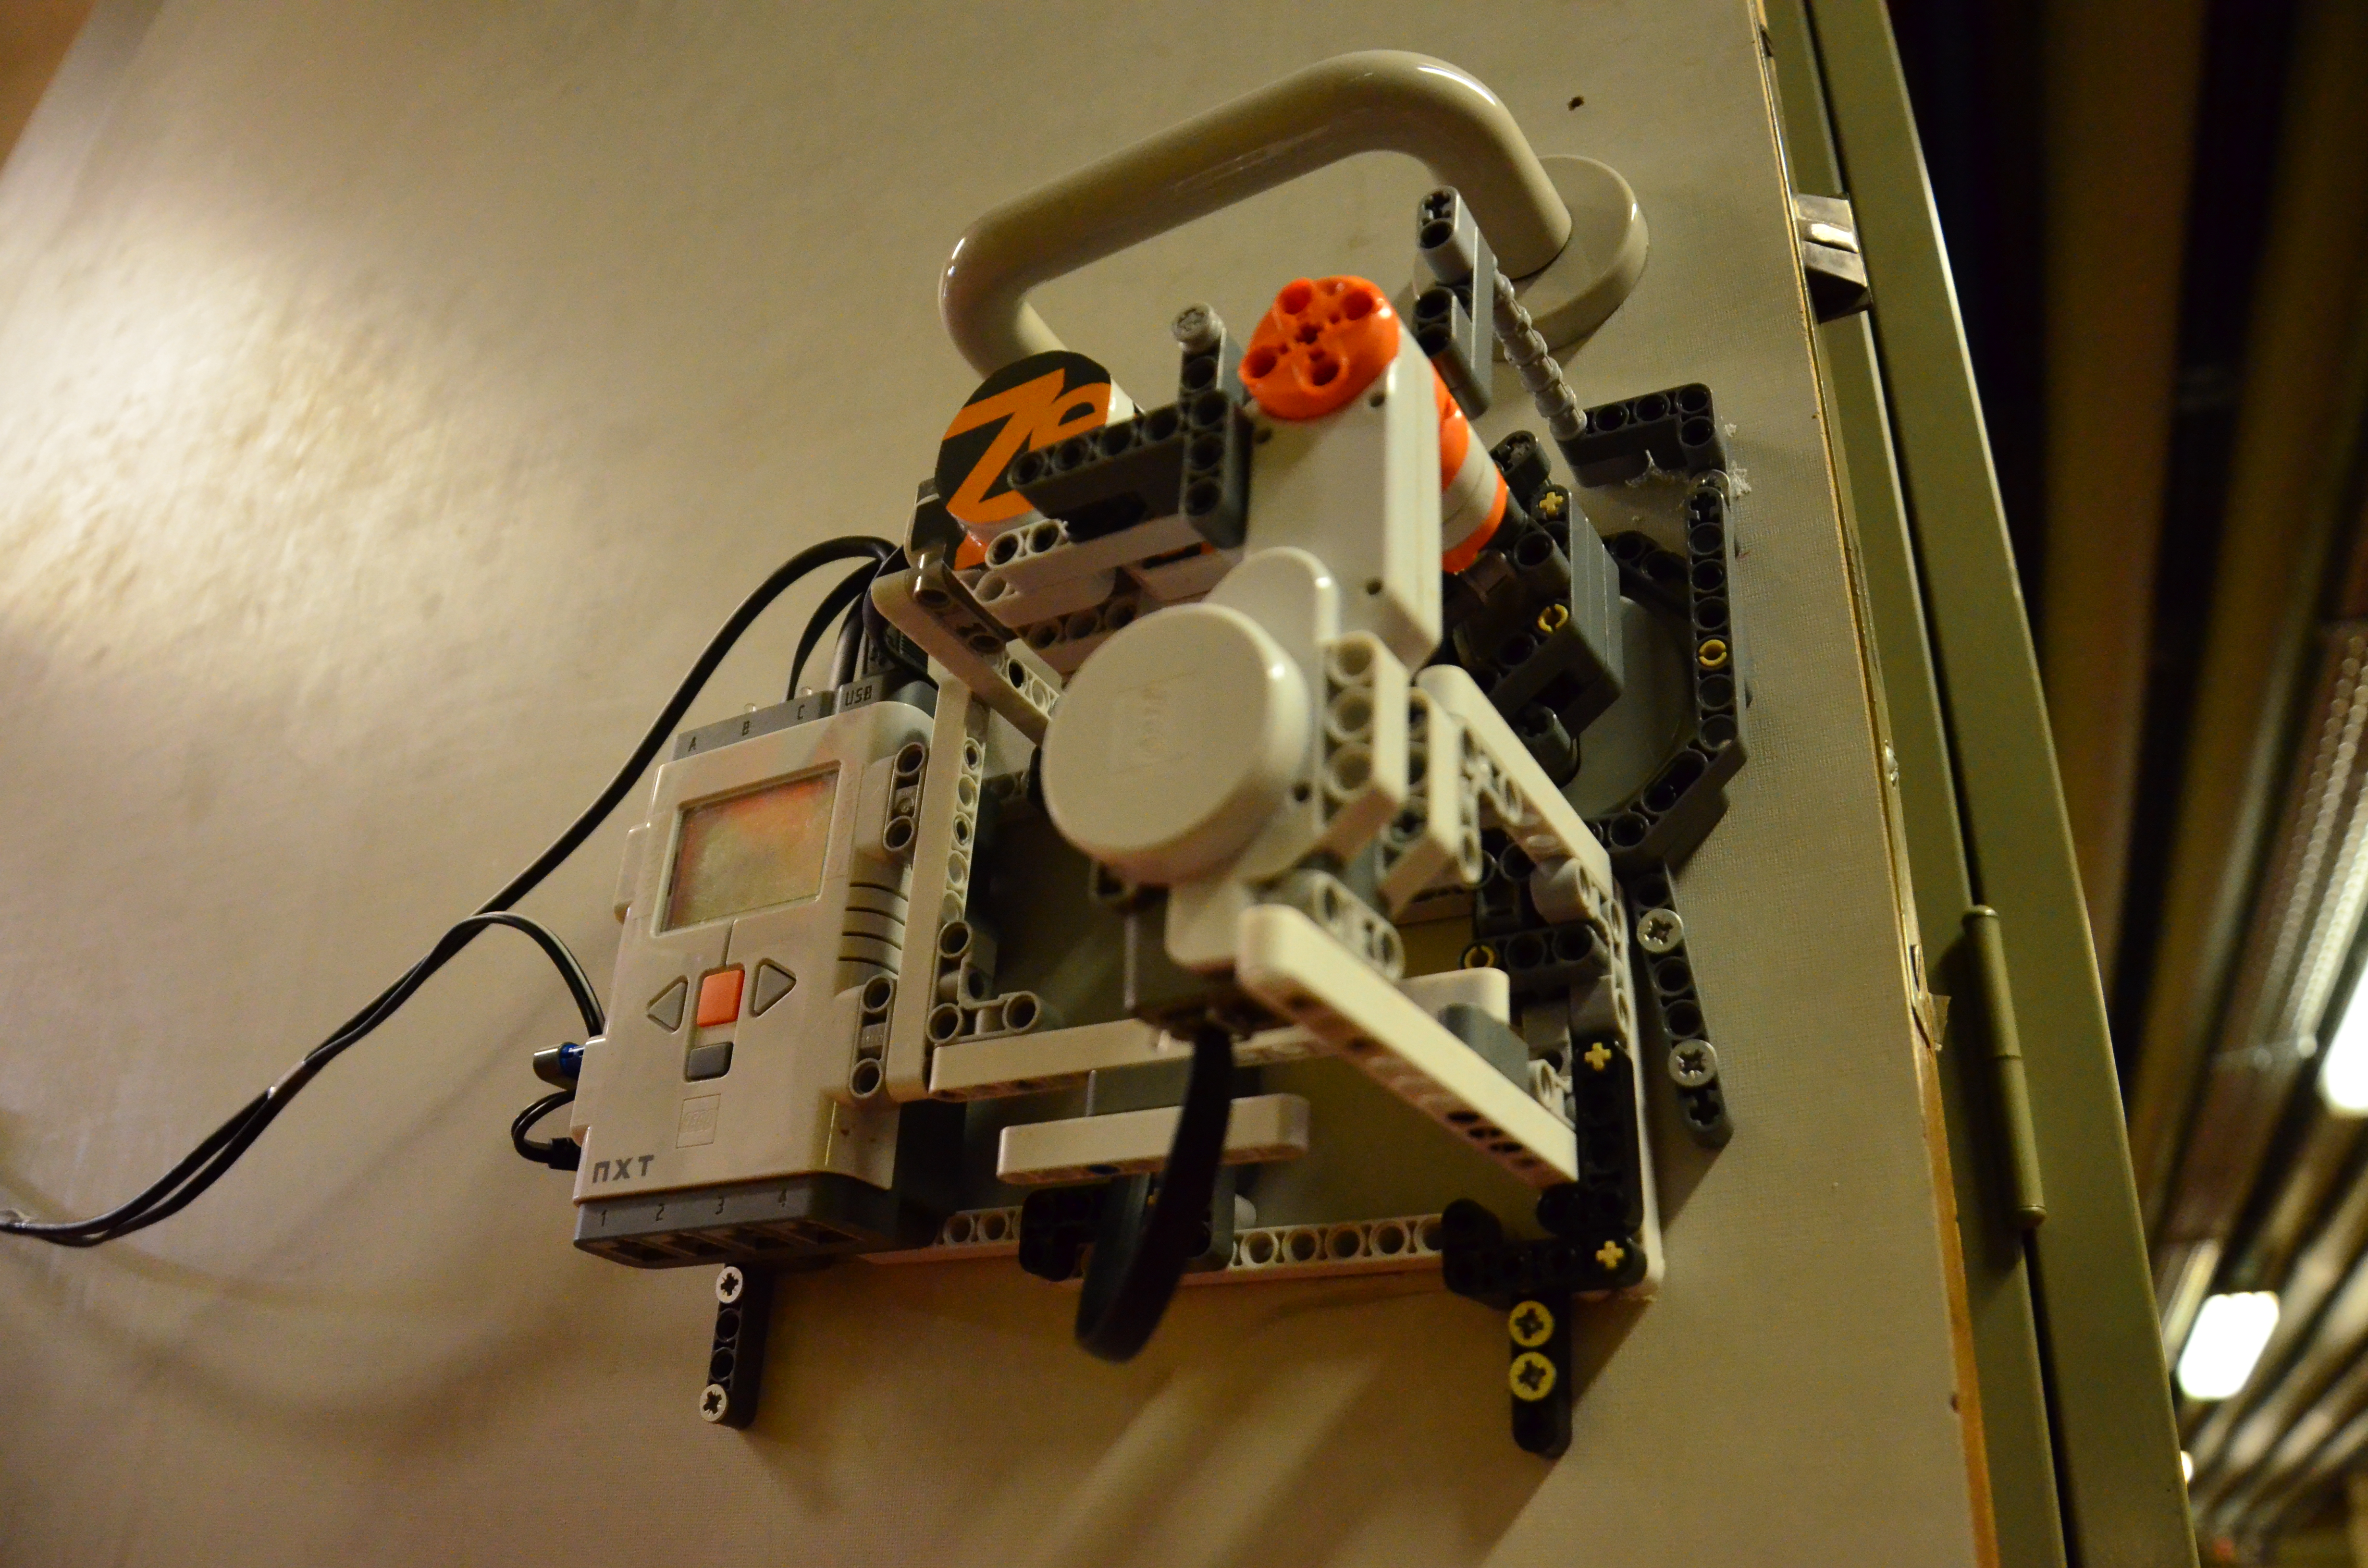
\includegraphics[width=180pt]{project_slotmachien}}}
  \end{textblock}
\end{frame}

\begin{frame}
  \begin{textblock}{60}(10,15)
    {\huge Gamification}
  \end{textblock}
  \begin{textblock}{20}(25,30)
    \visible{\fbox{\includegraphics[width=230pt]{project_gamification.png}}}
  \end{textblock}

\end{frame}

% Kelder
\begin{frame}
  \begin{center}
    {\Huge{Zeus Kelder}}\\[5mm]

    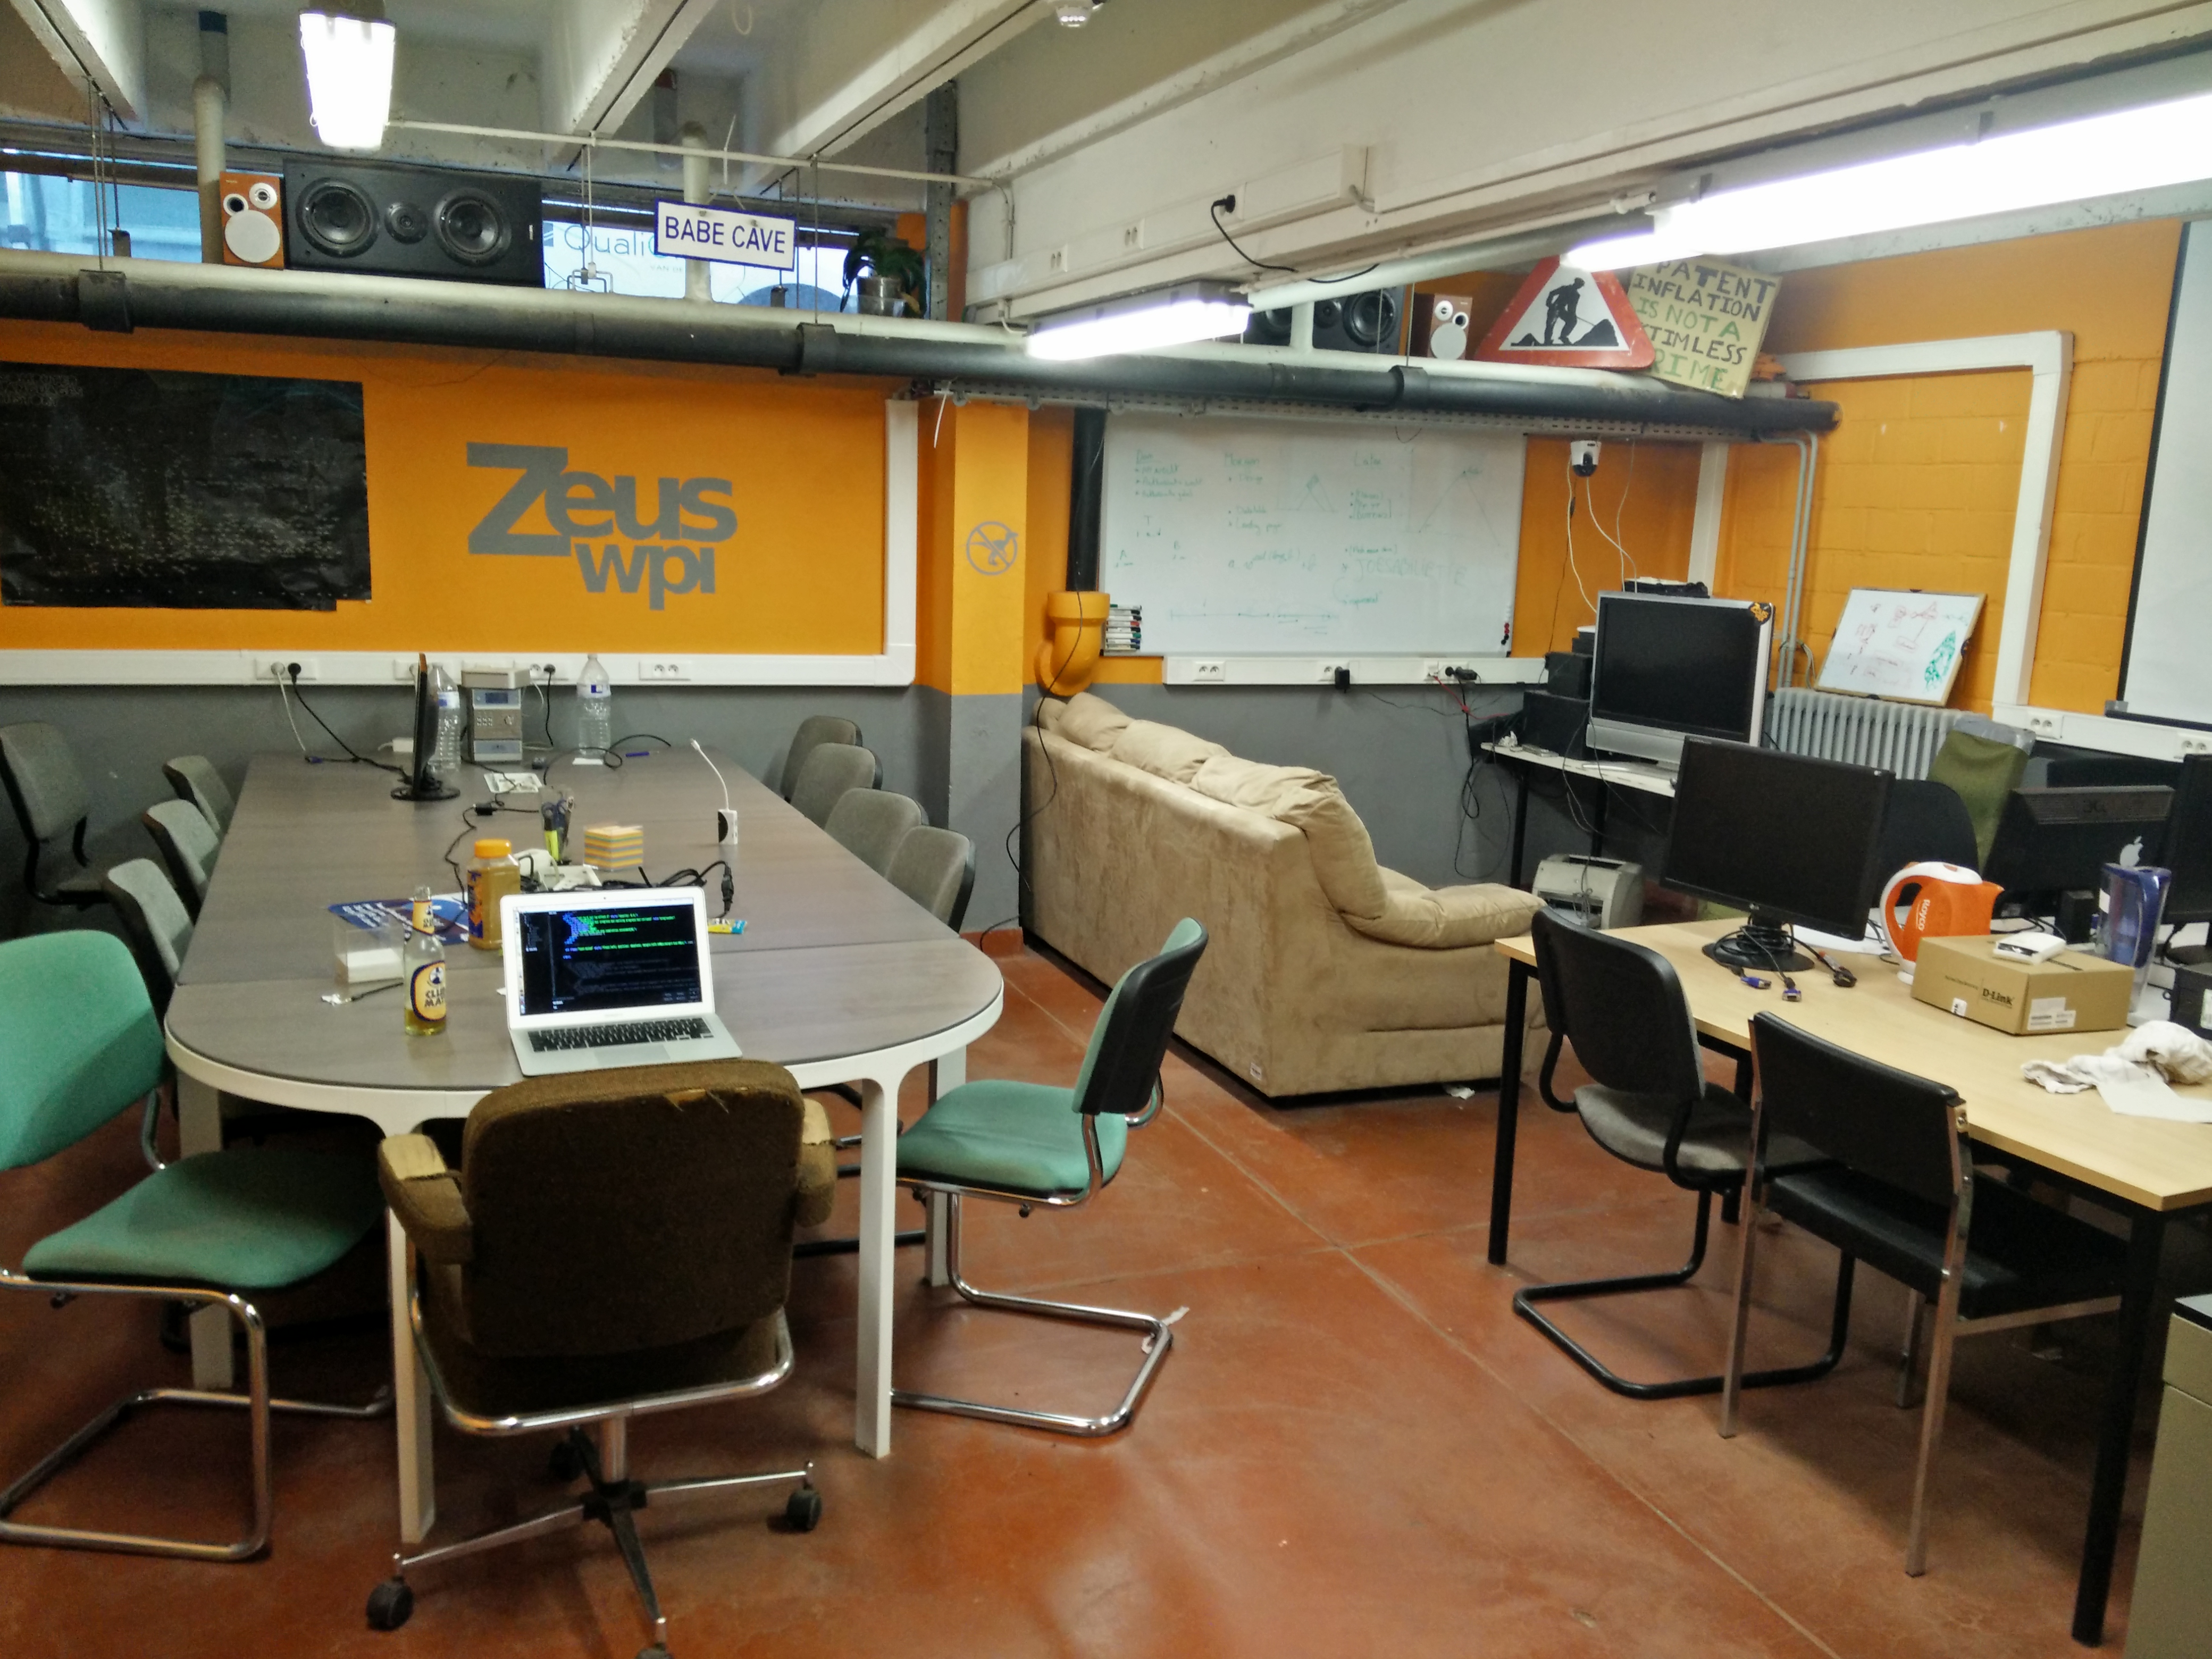
\includegraphics[width=250pt]{kelder.jpg}

    \bigskip 51.023102,3.710265 | Verdieping -1
  \end{center}

\end{frame}

\end{document}
